\section{}
% Consider the following closed-loop system:
% s+1
% s 10 2−4
% r y
% −
% e u
% (a) Using MATLAB, produce the Nyquist plot of L(s) for this system. Include a print-out of your
% plot.
% (b) Based on the plot in (a), explain why the closed-loop system is stable
% (c) Read off the GM, PM and t
% max
% d
% of the closed-loop system from the MATLAB-produced Nyquist
% plot
% (d) Set up a Simulink diagram of the above diagram, and employ a reference step input r(t) =
% 1+(t). Provide a print-out of the response y(t).
% (e) Now add a time delay of td = 0.1 s into the feedback loop, using the Transport Delay block
% within the Continuous part of the Simulink library. Using the same reference as in (d), provide
% a print-out of the resulting response. How does this plot compare to the one in (d)?
% (f) Now increase the time delay to td = 0.5 s. Comment on the step response of the closed-loop
% system in this case. Is this as expected?

Consider the following closed-loop system:
\begin{figure}[h]
    \centering
    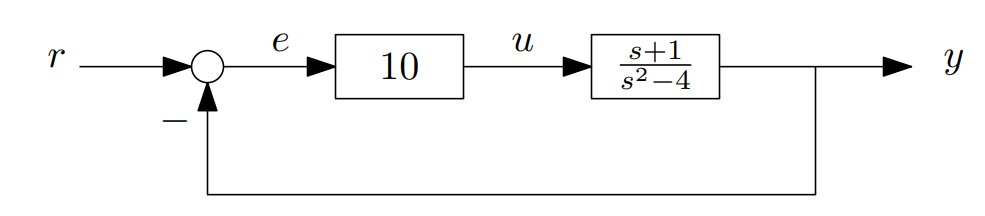
\includegraphics[width=0.5\textwidth]{Questions/Figures/Q3ProblemDiagram.png}
\end{figure}
\begin{enumerate}[label=(\alph*)]
    \item Using MATLAB, produce the Nyquist plot of $L(s)$ for this system. Include a print-out of your plot.
    \item Based on the plot in (a), explain why the closed-loop system is stable
    \item Read off the $GM$, $PM$ and $t_{max}$ of the closed-loop system from the MATLAB-produced Nyquist plot
    \item Set up a Simulink diagram of the above diagram, and employ a reference step input $r(t) = 1+(t)$. Provide a print-out of the response $y(t)$.
    \item Now add a time delay of $t_d = 0.1$ s into the feedback loop, using the Transport Delay block within the Continuous part of the Simulink library. Using the same reference as in (d), provide a print-out of the resulting response. How does this plot compare to the one in (d)?
    \item Now increase the time delay to $t_d = 0.5$ s. Comment on the step response of the closed-loop system in this case. Is this as expected?
\end{enumerate}

\subsection{}
The loop function for this system is:
\begin{equation*}
    L(s) = \frac{10s + 10}{s^2-4}
\end{equation*}
By Matlab,
\begin{lstlisting}[language=Matlab]
nyquist(tf([10 10], [1 0 -4]))
\end{lstlisting}
\begin{figure}[h]
    \centering
    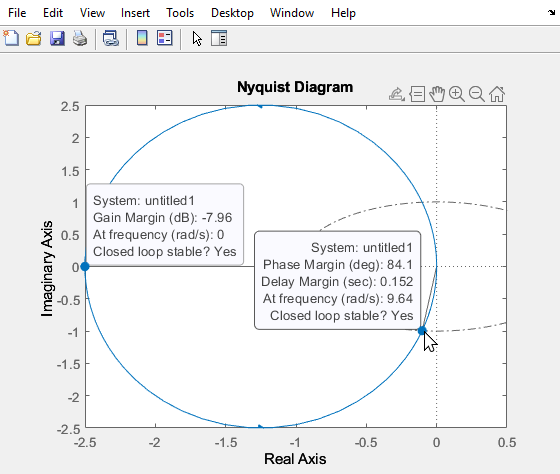
\includegraphics[width=0.5\textwidth]{Questions/Figures/Q3a.png}
    \caption{3(a) Nyquist plot generated by MATLAB}
\end{figure}

\subsection{}

The poles of $L(s)$ are at $s = \pm 2$. Then, $n = 1$. Since the Nyquist plot does not pass through $-1$ and encircles the origin once in the 
counter-clockwise direction, the closed-loop system is stable.

\subsection{}
\begin{verbatim}
>> db2mag(-7.96)

ans =

    0.3999
\end{verbatim}
then,
\begin{empheq}[box=\fbox]{align*}
    GM &= 0.3999 \\
    PM &= 84.1^\circ \\
    t_{d}^{max} &= 0.152 \text{ s}
\end{empheq}

\subsection{}
\begin{figure}[h]
    \centering
    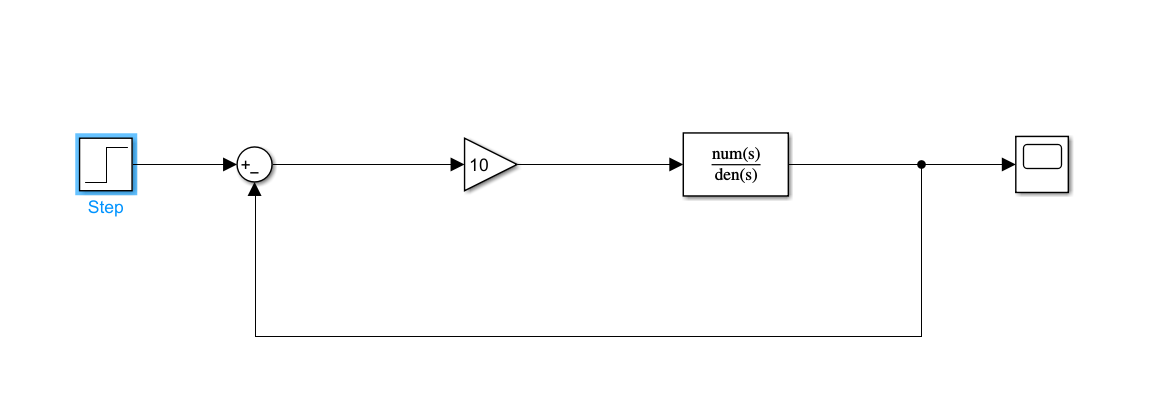
\includegraphics[width=0.5\textwidth]{Questions/Figures/Q3dSimulink.png}
    \caption{3(d) Simulink diagram}
\end{figure}

\begin{figure}[h]
    \centering
    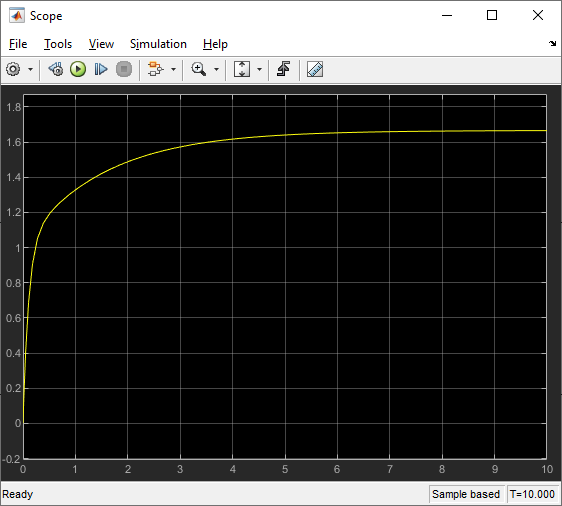
\includegraphics[width=0.5\textwidth]{Questions/Figures/Q3dScope.png}
    \caption{3(d) $y(t)$ response}
\end{figure}
\FloatBarrier
\subsection{}
\begin{figure}[h]
    \centering
    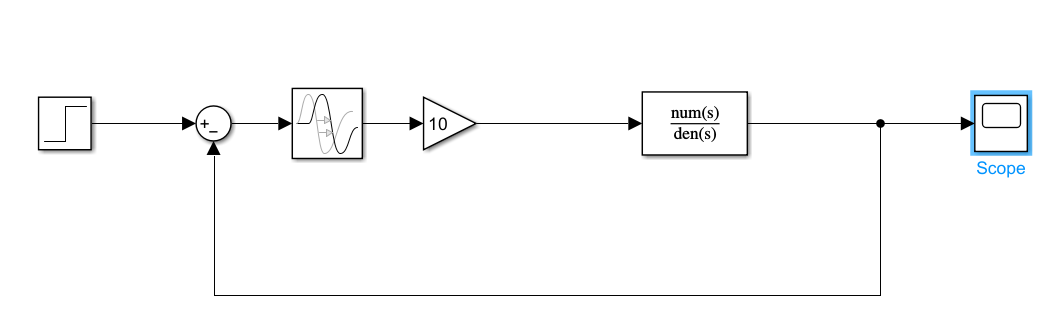
\includegraphics[width=0.5\textwidth]{Questions/Figures/Q3eSimulink.png}
    \caption{3(e) Simulink diagram}
\end{figure}
\begin{figure}[h]
    \centering
    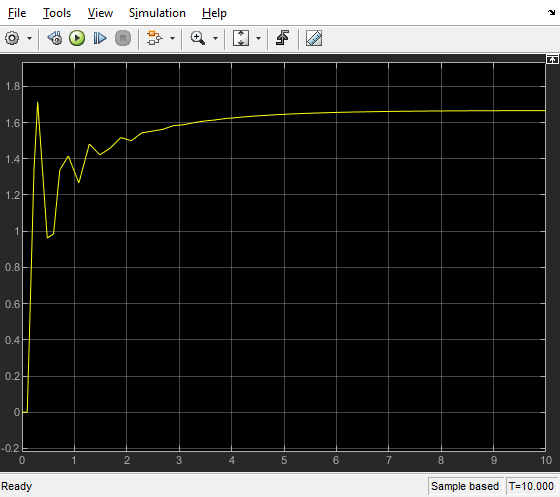
\includegraphics[width=0.5\textwidth]{Questions/Figures/Q3eScope.png}
    \caption{3(e) $y(t)$ response}
\end{figure}

The response is more oscillatory than in (d) initially. After some time they both converge to the same value.

\FloatBarrier
\subsection{}
\begin{figure}[h]
    \centering
    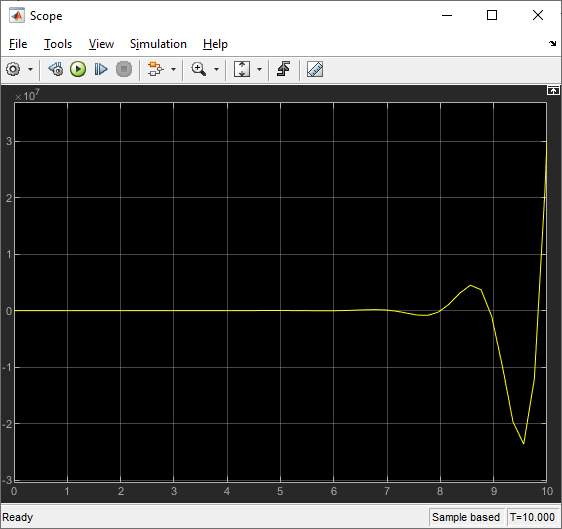
\includegraphics[width=0.5\textwidth]{Questions/Figures/Q3f.png}
    \caption{3(f) $y(t)$ response}
\end{figure}

The response blows up to $\infty$ as $t \to \infty$. This is expected since the system is unstable at $t_d = 0.5$ s as 
discussed in (b).